\documentclass[border=2mm]{standalone} 

\usepackage{graphicx}
\usepackage{siunitx}
\usepackage[siunitx]{circuitikz}

\begin{document} 

	\resizebox {\columnwidth} {!} { 
	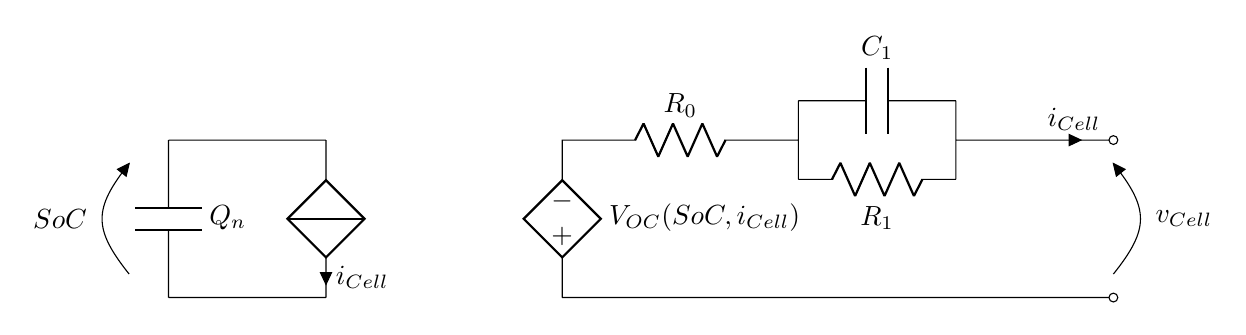
\begin{tikzpicture}[remember picture, european voltages, american currents]	
		\ ctikzset { bipoles/capacitor/voltage/ distance from node=10}
		\draw 
		
		% SoC
		(0,0) to[C, l_=$Q_n$] (0,2)
		(2,2) to[cI=$i_{Cell}$] (2,0) 
	   	(0,0) to[short] (2,0)
	   	(0,2) to[short] (2,2)
	   	
	   	(-0.5,0) to[open, v^>=$SoC$] (-0.5,2)
		
		% Controlled SoC
		(5,0) to[american controlled voltage source, l_=$V_{OC}({ SoC, i_{Cell} })$] 
		(5,2) to[R=$R_0$] (8,2) 

		% RC Loop 1
		(8,1.5) -- (8,2.5)	
		(8,1.5)to[R, l_=$R_1$] ( 10, 1.5)
		(8,2.5)to[C=$C_1$] ( 10, 2.5)
		(10,1.5) -- (10,2.5)

		(10, 2) -- (11, 2)
		
		% Cell current arrow
		(11,2) to[short,-o,i=$i_{Cell}$] (12,2)
		(12,2) node[anchor=west] {}
		
		(5,0) to[short,-o] (12,0) 		
		(12,0) node[anchor=west] {}

		% Cell voltage arrow
	    (12,0) to[open, v>=$v_{Cell}$] (12,2)

	;\end{tikzpicture}
	}

\end{document}